\subsection{Local systems and the Reidemeister trace}

Let $g\colon X\to X$ be a self-map of a compact anima $X$. Consider again the lax commutative square~\eqref{eq:lax-comm-square-lefschetz} from~\cref{sec: lefschetz theory}, which we viewed as a morphism in the category of traceable endomorphisms $\Endtrl(\Prlstf)$. If $g\colon X\to X$ happened to be induced by a self-map $f\colon\tset\to\tset$ for some well-behaved space $\tset$, we recovered the Lefschetz fixed point theorem for $f$ by factoring~\eqref{eq:lax-comm-square-lefschetz} through the object $(\D{\tset },f_!)\in\Endtrl(\Prlstf)$.

Putting topology aside for now, a more obvious factorization of~\eqref{eq:lax-comm-square-lefschetz} is through the category of local systems (aka parametrized spectra) $\Sp^X$:
\begin{prop}
  Let $g\colon X\to X$ be a self-map of a compact anima $X$. Considered as a morphism in $\Endtrl(\Prlstf)$, the lax commutative square~\eqref{eq:lax-comm-square-lefschetz} factors as
  \begin{equation}
    \label{eq:lax-composition-reidemeister}
    \left(
      \begin{tikzcd}[column sep=large]
        \Sp^X \arrow[r,"X_\sharp"] \arrow[d,"g^*"] & \Sp \arrow[d,equal]\\
        \Sp^X \arrow[r,swap,"X_\sharp"]  \arrow[ru,Rightarrow, shorten <=5pt,shorten >=5pt]  & \Sp
      \end{tikzcd}
    \right)
    \circ
    \left(
      \begin{tikzcd}[column sep=large]
        \Sp \arrow[r,"X^*"] \arrow[d,equal] & \Sp^X \arrow[d,"g^*"]\\
        \Sp \arrow[r,swap,"X^*"] & \Sp^X
      \end{tikzcd}
    \right),
  \end{equation}
  where the rightmost square $2$-cell is the invertible one coming from functoriality of pullback, and the leftmost $2$-cell is the counit transformation $X_\sharp g^*\simeq X_\sharp g_\sharp g^*\to X_\sharp$.
\end{prop}
\begin{proof}
  Aside from the usual adjunctions $X_\sharp\dashv X^*\dashv X_*$, the fact that $X$ is compact furnishes an additional adjunction $X_*\dashv \Hom_{\Sp^X} (D_X,X^*({-}))$, where $D_X$ is the dualizing object of $X$. It follows that the horizontal morphisms in both squares are strongly continuous, and hence that they define morphisms in $\Endtrl(\Prlstf)$. Concatenating the two $2$-cells recovers the one in~\eqref{eq:lax-comm-square-lefschetz} on the nose.
\end{proof}
As in the previous section, we then get
\begin{cor}\label{cor: reidemeister lefschetz triangle}
  For a self-map $g\colon X\to X$ of a compact anima $X$, there is a commutative diagram
  \begin{equation}
    \label{eq:reidemeister-lefschetz-triangle}
    \begin{tikzcd}[column sep=tiny]
      & \tr{g^*\curvearrowright\Sp^X}{}\arrow[dr] \\
      \SS\arrow[rr]\arrow[ru] && \SS,
    \end{tikzcd}
  \end{equation}
  where the bottom arrow is the Lefschetz trace of $g$.
\end{cor}
Just as in the previous section, the axioms of six-functor formalisms allow us to quickly compute the trace $\tr{g^*\curvearrowright\Sp^X}{}$ with the suspension spectrum of a space of ``fixed points'' for the map $g$. Here fixed points must be interpreted in a homotopy-invariant way; we let $\cL^gX$ denote the homotopical fixed point space defined to be the homotopy pullback
\[
  \begin{tikzcd}
    \cL^{g}X  & X \\
    X & X\times X\,.
    \arrow[from=1-1, to=1-2]
    \arrow["\lrcorner",phantom,very near start, from=1-1, to=2-2]
    \arrow[from=1-1, to=2-1]
    \arrow["\Delta", from=1-2, to=2-2]
    \arrow["\Gamma^g"', from=2-1, to=2-2]
  \end{tikzcd}
\]
That is, we have
\begin{lem}\label{lem: reidemeister trace computation}
  Let $g\colon X\to X$ be a self-map of a compact anima. There is an equivalence of spectra
  \[
    \tr{g^*\curvearrowright\Sp^X}{}\simeq\SS\lbrack\cL^{g}X\rbrack,
  \]
  natural in intertwining maps $h\colon (X,g)\to (X',g')$. 
\end{lem}
\begin{proof}
  The identification comes about exactly as in the proof of~\cref{lem: trace computation}. Unlike in the topological setting, we do not need to require anything of $h$ beyond being an intertwining map, since any intertwining map induces a morphism
  \begin{equation}
    \label{eq:square-induced-by-proper-morphism}
    \begin{tikzcd}
      \Sp^{X}\arrow[r,"h_\sharp"]\arrow[d,"g^*"]
      & \Sp^{X' }\arrow[d,"(g')^*"]\\
      \Sp^{X}\arrow[r,"h_\sharp"]\arrow[ru,Rightarrow, shorten <=5pt,shorten >=5pt]
      & \Sp^{X'}
    \end{tikzcd}
  \end{equation}
  in $\Endtrl(\Prlstf)$, where the $2$-cell is the Beck--Chevalley morphism.
\end{proof}
Combining~\cref{lem: reidemeister trace computation} with~\cref{cor: reidemeister lefschetz triangle}, we find
\begin{thm}
  Let $g\colon X\to X$ be a self-map of a compact anima. There is a commutative triangle
  \begin{equation}
    \label{eq:reidemeister-lefschetz-triangle-with-identification}
    \begin{tikzcd}[column sep=tiny]
      & \SS\lbrack\cL^{g}X\rbrack\arrow[dr] \\
      \SS\arrow[rr]\arrow[ru] && \SS,
    \end{tikzcd}
  \end{equation}
  in which the bottom arrow is the Lefschetz trace and the arrow $\SS\lbrack\cL^{g}X\rbrack\to\SS$ is induced by the projection $\cL^{g}X\to\pt$.
\end{thm}
\begin{proof}
  The second statement follows from the naturality of the identification in~\cref{lem: reidemeister trace computation}.
\end{proof}
We have constructed a homotopy invariant for self-maps that refines the Lefschetz trace:
\begin{defn}
  The map $\mdef{\rho_g}\colon \SS\to\SS\lbrack\cL^{g}X\rbrack$ in~\eqref{eq:reidemeister-lefschetz-triangle-with-identification} is the
  \tdef{Reidemeister trace} of $g$.
\end{defn}

\subsection{Factoring the Reidemeister trace using cosheaves}

Let $\tset\in \Top$ be compact and locally of singular shape with
associated anima $\ani{\tset}\tset$. Given some self map
$f\colon\tset\to\tset$, we can now associated two different invariants
to this datum, namely the topological Reidemeister trace
\[ \lambda_f\colon \SS \to \Sections{\tset;\omega_\tset}\,,\]
as well as its homotopical counterpart:
\[ \rho_{f}\colon \SS \to \SS [\cL^{f}\ani{\tset}]\,.\]
The insight is that the Lefschetz--Nielsen theorem \todo{Add ref},
will be an immediate consequence of relating these two invariants.
More precisely, we show:

\begin{thm}
    Let $\tset \in \Top$ be compact and locally of singular shape. 
    Then we have a commutative diagram in the category of spectra:
    \[\begin{tikzcd}
	& {\Sections{\tset,\omega_{\tset}}} \\
	\SS & {\SS[\cL^f\ani{\tset}]}
	\arrow["{\mathfrak{a}}", from=1-2, to=2-2]
	\arrow["{\lambda_f}", from=2-1, to=1-2]
	\arrow["{\rho_f}"', from=2-1, to=2-2]
\end{tikzcd}\]
which is natural in intertwining maps.
\end{thm}

In the spirit of fixed point theory, we would like to relate the Reidemeister trace of $g$ to the actual fixed point space $\tset^f$. We do so by following the pattern of~\cref{sec: lefschetz theory}. First, then, we should factor the square
\begin{equation}
  \label{eq:lax-comm-square-reidemeister}
  \begin{tikzcd}[column sep=large]
    \Sp \arrow[r,"X^*"] \arrow[d,equal] & \Sp^X \arrow[d,"g^*"]\\
    \Sp \arrow[r,swap,"X^*"] & \Sp^X
  \end{tikzcd}
\end{equation}
through an object in $\Endtrl(\Prlstf)$ that has access to actual topological information about the pair $(A,f)$. Such a factorization is achieved by the {\em assembly functor} of Bartels and Nikolaus. Although this work is the subject of a still unpublished article, an expository account can be found in the lecture notes~\cite{Nikolaus2024}.
\begin{defn}[Bartels--Nikolaus]\label{defn: abstract assembly}
  Let $(\mathcal C,\otimes ,1)$ be a closed symmetric monoidal category with internal mapping object $\Hom_{\mathcal C}({-},{-})$. Given objects $A$ and $B$ in $\mathcal C$ together with a map 
  \[
    \delta\colon 1\to A\otimes B,
  \]
  the associated {\em $\delta$-assembly map}, denoted $a_\delta$, is defined by the following string diagram 
  \begin{equation*}
    \label{eq:abstract-assembly}
    a_\delta =
    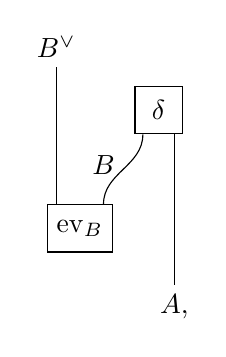
\begin{tikzpicture}[baseline=(current bounding box.center)]
      % Nodes
      \node (Bvee) at (-0.3,3.3) {$B^\vee$};
      \node (deltabox) at (1,2.5) [rectangle, draw, minimum width=0.6cm, minimum height=0.6cm] {$\delta$};
      \node (evbox) at (0,1) [rectangle, draw, minimum width=0.6cm, minimum height=0.6cm] {$\mathrm{ev}_B$};
      \node (A) at (1.2,0) {$A$,};
      \node (B) at (0.3,1.8) {$B$};

      % Edges
      \draw (Bvee) -- (evbox.north -| -0.3,1.3);
      \draw (deltabox.south -| 0.8,2.5) to [out=270,in=90] (evbox.north -| 0.3,1.3);
      \draw (deltabox.south -| 1.2,2.5) -- (A);
    \end{tikzpicture}
  \end{equation*}
  where $B^\vee = \Hom_{\mathcal C}(B,1)$ and $\mathrm{ev}_B\colon B^\vee\otimes B\to 1$ is the evaluation map, i.e. the counit of the adjunction between ${-}\otimes B$ and $\Hom_{\mathcal C}(B,{-})$.
\end{defn}
Let $\Prdual$ denote the category of dualizable stable categories with strongly continuous functors between them. The Lurie tensor product on presentable categories restricts to a symmetric monoidal structure on $\Prdual$. By \cite{Ramzi2024}, this symmetric monoidal structure is closed. We denote the resulting internal mapping object by $\Homd ({-},{-})$.
\begin{defn}[Bartels--Nikolaus]
  Let $\tset$ be a locally compact Hausdorff space. The category of \tdef{completed cosheaves} on $\tset$, denoted $\coShat (\tset )$, is given by
  \[
    \coShat (\tset ) = \Homd (\D{\tset},\Sp ).
  \]
\end{defn}
Although general objects of $\coShat (\tset )$ are quite mysterious, the definition does give us a description of the compact objects via
\[
  \coShat (\tset )^\omega\simeq\Map_{\Prdual}(\Sp ,\coShat (\tset ))
  \simeq\Map_{\Prdual}(\Sp,\Homd (\D{\tset},\Sp ))\simeq\Map_{\Prdual}(\D{\tset},\Sp),
\]
where the final equivalence used the adjunction between internal mapping object and $\otimes$. That is, the groupoid of compact objects $\coShat (\tset )^\omega$ is equivalent to the groupoid strongly continuous functors $\D{\tset}\to\Sp$, which is a subgroupoid of the more familiar groupoid of all colimit-preserving functors $\D{\tset}\to\Sp$. Of particular interest is the strongly continuous functor
\[
\tset_\sharp\colon\D{\tset}\to\Sp
\]
that is left adjoint to $\tset^*$, defined if $\tset$ is locally of singular shape. The corresponding compact object of $\coShat (\tset )$ is denoted $w_\tset$ and referred to as the \tdef{local Wall object} of $\tset$.

Another aspect of $\coShat (\tset )$ which is well-understood by hard work of Bartels--Nikolaus and Efimov is its value under localizing invariants:
\begin{thm}[Bartels--Efimov--Nikolaus]\label{thm: K theory of completed cosheaves}
  $K(\coShat (\tset ))\simeq \tset_*\tset^!K (\SS )$.
\end{thm}
Finally, we will need to introduce some notation for the functoriality of $\coShat (\tset )$. If $h\colon\tset\to\tset '$ is a proper map of locally compact Hausdorff spaces, we get as usual that the pullback $h^*\colon\D{\tset '}\to \D{\tset}$ is strongly continuous. Hence it induces a map on completed cosheaves that we denote
\[
h_?\colon \coShat (\tset )\to \coShat (\tset ').
\]
That is, the category of completed cosheaves is {\em covariantly functorial in proper maps}. Since $h_?$ is strongly continuous by construction, it admits a colimit-preserving left adjoint that we denote
\[
h^?\colon \coShat (\tset ')\to \coShat (\tset ).
\]
The reader may observe that there is an additional contravariant functoriality in etale maps, for instance, that one would might want to denote $h^{\text{?`}}$.


\medskip

Assume that $\tset$ is locally of singular shape and compact. Under these assumptions, we have a sequence of colimit-preserving functors
\[
  \D{\tset}\otimes\Sp^{\fundgroupoid (\tset )}\xrightarrow{\id\otimes\psi^*}
  \D{\tset}\otimes \D{\tset}\xrightarrow{\Delta^*}\D{\tset}\xrightarrow{\tset^*}
  \Sp, 
\]
where $\psi^*\colon \Sp^{\fundgroupoid (\tset )}\to\D{\tset}$ denotes the inclusion of local systems into all sheaves. Bartels and Nikolaus show that the composite $\D{\tset}\otimes\Sp^{\fundgroupoid (\tset )}\to\Sp$ admits a left adjoint
\[
\delta\colon \Sp\to \D{\tset}\otimes\Sp^{\fundgroupoid (\tset )},
\]
which is then a strongly continuous functor and thus a morphism in the category $\Prdual$. Specializing~\cref{defn: abstract assembly} to this situation, we thus get a strongly continuous functor
\begin{equation}
  \label{eq:BN-assembly}
  a_\delta\colon\coShat (\tset )\to \Sp^{\fundgroupoid (\tset )},
\end{equation}
the \tdef{Bartels--Nikolaus assembly functor}.
\begin{thm}[Bartels--Nikolaus]\label{thm: Bartels--Nikolaus geometric topology}
  Let $\tset$ be a compact Hausdorff space that is locally of constant shape.
  Then the functor~\eqref{eq:BN-assembly}
  \begin{enumerate}[label=(\roman*)]
  \item induces the Waldhausen assembly map on $K$-theory and
  \item maps the local Wall object $w_\tset$ to the constant sphere spectrum $\SS_{\fundgroupoid \tset}$.
  \end{enumerate}
\end{thm}
Part (ii) means that we can factor $(\fundgroupoid\tset )^*\colon\Sp\to\Sp^{\fundgroupoid\tset}$ through the Bartels--Nikolaus assembly functor. Better, we have
\begin{prop}
  Let $f\colon \tset\to \tset$ be a self-map of a compact Hausdorff space that is locally of singular shape. Considered as a morphism in $\Endtrl(\Prlstf)$, the lax commutative square~\eqref{eq:lax-comm-square-reidemeister} factors as
  \begin{equation}
    \label{eq:lax-composition-cosheaves}
    \left(
      \begin{tikzcd}[column sep=large]
        \coShat (\tset ) \arrow[r,"a_\delta"] \arrow[d,"f^?"] & \Sp^{\fundgroupoid (\tset )} \arrow[d,"f^*"]\\
        \coShat (\tset ) \arrow[r,swap,"a_\delta"] \arrow[ru,Rightarrow, shorten <=5pt,shorten >=5pt]  & \Sp^{\fundgroupoid (\tset )}
      \end{tikzcd}
    \right)
    \circ
    \left(
      \begin{tikzcd}[column sep=large]
        \Sp \arrow[r,"w_\tset"] \arrow[d,equal] & \coShat (\tset ) \arrow[d,"f^?"]\\
        \Sp \arrow[r,swap,"w_\tset"]  \arrow[ru,Rightarrow, shorten <=5pt,shorten >=5pt]  & \coShat (\tset )
      \end{tikzcd}
    \right),
  \end{equation}
  in which the leftmost $2$-cell is the transpose of the commutative diagram
  \[
    \begin{tikzcd}[column sep=large]
      \coShat (\tset ) \arrow[r,"a_\delta"] \arrow[d,"f_?"] & \Sp^{\fundgroupoid (\tset )} \arrow[d,"f_!"]\\
      \coShat (\tset ) \arrow[r,swap,"a_\delta"]   & \Sp^{\fundgroupoid (\tset )}
    \end{tikzcd},
  \]
  and the rightmost $2$-cell is the transpose of the $2$-cell
  \[
    \begin{tikzcd}[column sep=large]
      \Sp \arrow[r,"w_\tset"] \arrow[d,equal] & \coShat (\tset ) \arrow[d,"f_?"]\\
      \Sp \arrow[r,swap,"w_\tset"]  \arrow[ru,Leftarrow, shorten <=5pt,shorten >=5pt]  & \coShat (\tset )
    \end{tikzcd}
  \]
  coming from the counit transformation
  \[
    f_?(w_\tset) = \tset_\sharp\circ f^*\simeq\tset_\sharp \circ f_\sharp\circ f^*\to\tset_\sharp = w_\tset.
  \]
\end{prop}
\begin{cor}
  Let $f\colon \tset\to \tset$ be a self-map of a compact Hausdorff space that is locally of singular shape. There is a commutative triangle
  \begin{equation}
    \label{eq:nielsen-triangle-without-identification}
    \begin{tikzcd}[column sep=tiny]
      & \tr{f^?\curvearrowright\coShat (\tset )}{}\arrow[dr] \\
      \SS\arrow[rr]\arrow[ru] && \SS\lbrack\cL^{f}\fundgroupoid\tset\rbrack,
    \end{tikzcd}
  \end{equation}
  where the bottom horizontal arrow is the Reidemeister trace.
\end{cor}
\subsection{Another trace ``calculation''}
Keeping with the pattern laid out in~\cref{sec: lefschetz theory}, the next step in our treatment of Lefschetz--Nielsen theory is a calculation of the categorical trace that shows up as the apex in the triangle~\eqref{eq:nielsen-triangle-without-identification}. Unlike in the Lefschetz and Reidemeister trace incarnations of this step, we will not be able to calculate $\tr{f^?\curvearrowright\coShat (\tset )}{}$ in the strict sense (without a big effort); instead, we will give a lax calculation that suffices for the purposes of fixed point theory. This idea is again adapted to our setting from unpublished work of Bartels and Nikolaus, who show using simple manipulations in closed monoidal categories that the map induced on $K$-theory by their assembly functor $a_\delta\colon\coShat (\tset )\to \Sp^{\fundgroupoid (\tset )}$ factors through $\tset_*\tset^!K\SS$, thereby removing the difficult~\cref{thm: K theory of completed cosheaves} from the dependencies of the customer-facing~\cref{thm: Bartels--Nikolaus geometric topology}.

We should expect the calculation of $\tr{f^?\curvearrowright\coShat (\tset )}{}$ to be difficult, because for $f=\id$ it is already a difficult theorem of Efimov.\todo{motivate linearizing over free algebra on dualizable generator}
\begin{defn}[The free algebra on one dualizable object]
  $\freeondual = \Fun (\mathrm{Bord}^1_{\mathrm{fr}}(\RR^1)^{\op},\Sp )$\todo{define Hopf algebra structure}
\end{defn}
 
% \newpage

% Let $\Spc$ denote the $\infty$-category of spaces. For any $X \in \Spc$, we write
% $\Sp^{X}$ for the category of local systems of spectra on $X$. For any map of spaces
% $f\colon X \to Y$, the pullback functor $f^{\ast}\colon \Sp^Y\to \Sp^X$ admits both adjoints
% $f_{\sharp}\dashv f^{\ast} \dashv f_{\ast}$, given by left and right Kan extension respectively.
% As before, if $Y=\pt$ and $f$ is the terminal map, we also write $X^{\ast}=f^{\ast}$ and so on.
% With this notation, we have that the composite
% \[X_{\sharp}X^{\ast}\SS = \SS[X] = \colim_X \SS\]
% is given by the spherical chains on $X\in \Spc$.
% By \todo{CITE}, the assignment taking
% a span of spaces $X\xleftarrow{f}Y \xrightarrow{g} Z$ to the composite functor
% $\Sp^X \xrightarrow{f^{\ast}} \Sp^Y \xrightarrow{g_{\sharp}} \Sp^Z$ refines to a symmetric monoidal
% functor
% \[ (\Sp^{(-)})^{\ast}_{\sharp}\colon \Span{\Spc} \too \Prlst\,.\]
% Given a self map $f\colon X\to X$ of a space $X\in \Spc$, we write $\cL^{f}X$ for the pullback
% \[\begin{tikzcd}
%     \cL^{f}X  & X \\
%     X & X\times X\,.
%     \arrow[from=1-1, to=1-2]
%     \arrow[from=1-1, to=2-1]
%     \arrow["\Delta", from=1-2, to=2-2]
%     \arrow["\Gamma^f"', from=2-1, to=2-2]
%   \end{tikzcd}\]
% Note that, $\cL X = \cL^{\id}X= \Map(S^1,X)$ is simply the free loop space of $X$. Arguing as in
% the proof of \cref{lem: trace computation}, we immediately learn that
% \[ \tr{f^{\ast}\colon \Sp^X\to \Sp^X}{\L}\simeq \SS[\cL^{f}X] \in \Sp\,.\]

% In what follows, fix a self map $f\colon X\to X$ of a compact space $X\in \Spc^{\omega}$

% \begin{prop}\label{prop: weak lefschetz homotopical}
%   The trace $\tr{\SS[f]}{}\colon \SS\to \SS$ factors through the pushforward
%   $\SS[\cL^{f}X] \to \SS$ induced by the terminal map $\cL^{f}X\to \pt$.
% \end{prop}
% \begin{proof}
%   Since $X$ is compact, we have a chain of adjoints
%   $X_{\sharp} \dashv X^{\ast} \dashv X_{\ast} \dashv X^!$, so that $X_{\sharp}$ and $X^{\ast}$
%   are both strongly continuous. Let $\tau\colon X_{\sharp} f^{\ast}\to X_{\sharp}$ be the natural
%   transformation obtained by whiskering the counit $f_{\sharp}f^{\ast} \to \id_{\Sp^X}$ with
%   $X_{\sharp}$. Moreover, writing $\can \colon X^{\ast}\xrightarrow{\sim}f^{\ast}X^{\ast}$ for
%   the natural equivalence, we obtain a diagram in $\Endtrl(\Prlstf)$ of the form:
%   \[\begin{tikzcd}
%       {\Sp} & {\Sp^X} & {\Sp} \\
%       {\Sp} & {\Sp^X} & {\Sp}
%       \arrow["{X^{\ast}}", from=1-1, to=1-2]
%       \arrow[equals, from=1-1, to=2-1]
%       \arrow["{X_{\sharp}}", from=1-2, to=1-3]
%       \arrow["f^{\ast}",from=1-2, to=2-2]
%       \arrow[equals, from=1-3, to=2-3]
%       \arrow["\mathrm{can}"', Rightarrow, from=2-1, to=1-2]
%       \arrow["{X^\ast}"', from=2-1, to=2-2]
%       \arrow["{\tau}"', Rightarrow, from=2-2, to=1-3]
%       \arrow["{X_{\sharp}}"', from=2-2, to=2-3]\,.
%     \end{tikzcd}\]
%   Unwinding the definitions, we see that the composite is a map $(\Sp,\id)\to (\Sp,\id)$ given
%   by tensoring with the spectrum $\SS[X]$, together with the natural endomorphism of
%   $-\otimes \SS[X]$ given by the pushforward map $\SS[f]\colon \SS[X] \to \SS[X]$. Thus,
%   applying the functor $\TrcL$ to the diagram above, we obtain a commutative diagram
%   in spectra
%   \[\begin{tikzcd}
%       & {\tr{f^{\ast}}{\L}} \\
%       \SS && \SS
%       \arrow["{\TrcL(X_{\sharp},\tau)}", from=1-2, to=2-3]
%       \arrow["{\TrcL(X^{\ast},\can)}", from=2-1, to=1-2]
%       \arrow["{\tr{\SS[f]}{}}"', from=2-1, to=2-3]\,,
%     \end{tikzcd}\]
%   so it suffices to show that, under the identification $\tr{f^{\ast}}{\L} \simeq \SS[\cL^{f}X]$
%   the map $\TrcL(X_{\sharp},\tau)$ is given by the pushforward along the terminal map,
%   which again follows exactly as in \cref{lem: trace computation}
% \end{proof}

% \begin{defn}
%   Given a self map of a compact space $f\colon X\to X$, 
%   we denote the homology class factoring the trace obtained in
%   \cref{prop: weak lefschetz homotopical} by
%   \[ \mdef{\rho_f} \colon \SS\to \SS[\cL^{f}X]\,,\]
%   and call $\rho_f$ the \tdef{Reidemeister trace} of $f$.
% \end{defn}

% \subsection{Cosheaves and assembly}

% For a locally compact Hausdorff space $\tset \in \Top$, we write
% \[ \ani{\tset}\coloneq \ani{\mathrm{Sing}_{\bullet}{\tset}} \in \Spc\]
% for the geometric realization of the singular complex of $\tset$.
% If $\tset$ is compact and suave, we have a natural identification
% \[ \Gamma(\tset;\omega_\tset) \simeq \SS[\ani{\tset}]\]
% of the global sections of the dualizing sheaf with the spherical chains on $\ani{\tset}$,
% which we thus simply denote $\SS[\tset]$. 

% We now relate the Lefschetz index of a map $f\colon \tset \to \tset$ to the Reidemeister
% trace of the induced map $\ani{f}\colon \ani{\tset} \to \ani{\tset}$. Denote by
% $i\colon \ani{A^f} \to \cL^{\ani{f}}\ani{A}$ the natural map induced by the assignment
% taking a fixed point $a\in A^f$ to the pair $(a,\mathrm{const}_a)$ were $\mathrm{const}_a$
% is the constant path $a\to f(a)=a$. 

% \begin{thm}
%   For any self map of a compact suave Hausdorff space $f\colon \tset \to \tset$,
%   the Reidemeister trace $\rho_{\ani{f}}$ factors naturally in $f$ through the Lefschetz trace,
%   i.e.~we have a commutative diagram in spectra of the form:
% \[\begin{tikzcd}
% 	& {\Sections{\tset^f;\omega_{\tset^f}}} \\
% 	\SS & {\SS[\cL^{f}\ani{\tset}]}
% 	\arrow[from=1-2, to=2-2]
% 	\arrow["{\ch{}{f}}", from=2-1, to=1-2]
% 	\arrow["{\rho_{\ani{f}}}"', from=2-1, to=2-2]
% \end{tikzcd}\]
% \end{thm}

% We prove this by constructing a factorization of the map
% $(\ani{\tset}^{\ast},\can)\colon (\Sp,\id)\to (\Sp^{\ani{\tset}},\abs{f}^{\ast})$ in
% the category $\Endtrl(\Prlstf)$.

% \begin{defn}
%   Denote by $\Prdualf$ the sub-$(\infty,2)$-category of $\Prlstf$ spanned by the dualizable objects
%   in $\Prlstf$ with strongly continuous functors between them.
% For any $\tset \in \Top$ we write
% \[ \coShat(\tset) \coloneq \map_{\Prdualf}(\D{\tset}, \Sp)\]
% for the weak dual of $\D{\tset}= \Shv(\tset; \Sp)$ in $\Prdualf$.
% \end{defn}
% Barthels--Nikolaus construct a factorization of the functor $\ani{\tset}^{\ast}\colon \Sp \to \Sp^{\ani{\tset}}$
% of the form
% \[ \Sp \xrightarrow{\chi_{\tset}^{\loc}} \coShat(\tset) \xrightarrow{\ass_{\tset}} \Sp^{\ani{\tset}}\,,\]
% where $\chi_{\tset}^{\loc}(\SS) $ is cosheaf taking an open $U\subseteq \tset$ to the spectrum
% $\SS[\abs{U}]$.

% \begin{prop}
% We have a natural factorization in $\Endtrl(\Prlstf)$ of the form:
% \[\begin{tikzcd}
% 	\Sp & {\coShat{\tset}} & {\Sp^{\ani{\tset}}} \\
% 	\Sp & {\coShat{\tset}} & {\Sp^{\ani{\tset}}}
% 	\arrow["{\chi_{\tset}^{\loc}}", from=1-1, to=1-2]
% 	\arrow["\id", from=1-1, to=2-1]
% 	\arrow["\ass_{\tset}", from=1-2, to=1-3]
% 	\arrow["{f^{\natural}}", from=1-2, to=2-2]
% 	\arrow["{f^{\ast}}", from=1-3, to=2-3]
% 	\arrow[ Rightarrow, from=2-1, to=1-2]
% 	\arrow["{\chi_{\tset}^{\loc}}"', from=2-1, to=2-2]
% 	\arrow[ Rightarrow, from=2-2, to=1-3]
% 	\arrow["\ass_{\tset}",from=2-2, to=2-3]
% \end{tikzcd}\]
% Moreover, the induced map on $\TrcL$ factors through $\TrcL(\D{\tset},f^{\ast})\simeq \Gamma_c(\tset;\SS_A)^{\vee}$. 
% \end{prop}



%%% Local Variables:
%%% mode: LaTeX
%%% TeX-master: "main"
%%% End:
